\chapter{Villarceau circles and Villarceau spheres}\label{ch:villarceau}

This chapter proves Theorem~\ref{thm:E} and Villarceau's theorem. The argument is the same for $d=2,4,8$: one fibre is computed explicitly, and the others are obtained from it by isometries that commute with stereographic projection. For octonions the only point that needs comment is that these isometries are left multiplications, which are orthogonal by \ref{D:norm}.

\section{Stereographic projection}\label{sec:stereo}

Fix $d\in\{2,4,8\}$ and a unit vector $\varepsilon\in\K$ with $\varepsilon\perp1$. For $v\in\K$ write $v_\varepsilon=\langle v,\varepsilon\rangle=\Re(v\bar\varepsilon)$ and $\pi(v)=v-v_\varepsilon\varepsilon\in\varepsilon^\perp$, the orthogonal projection onto the hyperplane $\varepsilon^\perp\subset\K$. Stereographic projection from the point $N=(0,\varepsilon)$ of $S^{2d-1}$ onto its tangent hyperplane at the antipode, translated to the origin, is
\begin{equation}\label{eq:sigmaN}
\sigma\colon S^{2d-1}\setminus\{N\}\to\K\times\varepsilon^\perp=\R^d\times\R^{d-1},\qquad
\sigma(A,B)=\frac{\bigl(A,\ \pi(B)\bigr)}{1-B_\varepsilon}.
\end{equation}
It is a conformal diffeomorphism, it maps round spheres not through $N$ to round spheres \cite{Lyo03}, and it commutes with every isometry of $\K^2$ that fixes $N$ and preserves the decomposition $\K\times\K$. For $d=2$ and $\varepsilon=i$,
\[
\sigma(z,w)=\frac{\bigl(z,\ \Re w\bigr)}{1-\Imag w}\in\C\times\R=\R^3 .
\]

For $0<a<1$ put $b=\sqrt{1-a^2}$ and $\Sigma_a=S^{d-1}(a)\times S^{d-1}(b)=\{(A,B):|A|=a,\ |B|=b\}\subset S^{2d-1}$. It does not contain $N$. Every point $(A,B)$ of $S^{2d-1}$ with $A\neq0\neq B$ lies on exactly one $\Sigma_a$, namely $a=|A|$, and $\Sigma_a=h_\K^{-1}\bigl(\{x_{d+1}=a^2-b^2\}\bigr)$ is the preimage of a sphere of latitude.

\begin{lemma}\label{lem:tube}
Let $R=1/a$ and $r=b/a$, so that $R^2-r^2=1$. Then $\sigma$ maps $\Sigma_a$ diffeomorphically onto the tube
\[
T_{R,r}=\bigl\{(x,y)\in\R^d\times\R^{d-1}:(|x|-R)^2+|y|^2=r^2\bigr\}.
\]
\end{lemma}

\begin{proof}
Let $(A,B)\in\Sigma_a$ and $\beta=B_\varepsilon\in[-b,b]$, so $|\pi(B)|^2=b^2-\beta^2$. For $(x,y)=\sigma(A,B)$ we have $|x|=a/(1-\beta)$ and $|y|^2=(b^2-\beta^2)/(1-\beta)^2$, hence
\[
a^2(1-\beta)^2\bigl((|x|-R)^2+|y|^2\bigr)=\bigl(a^2-(1-\beta)\bigr)^2+a^2(b^2-\beta^2)=(\beta-b^2)^2+a^2b^2-a^2\beta^2=b^2(1-\beta)^2,
\]
using $a^2-1=-b^2$ and $a^2+b^2=1$. So $(|x|-R)^2+|y|^2=b^2/a^2=r^2$. The restriction of $\sigma$ to $\Sigma_a$ is an injective immersion between compact connected manifolds of the same dimension $2d-2$, so it is a diffeomorphism onto $T_{R,r}$ by invariance of domain.
\end{proof}

For $d=2$, $T_{R,r}$ is the torus obtained by rotating the circle $(x_1-R)^2+x_3^2=r^2$ of the $(x_1,x_3)$-plane about the $x_3$-axis, a ring torus because $R>r$. For $d=4,8$ it is the boundary of the tubular neighbourhood of radius $r$ of the round sphere $S^{d-1}(R)\subset\R^d\times0$, diffeomorphic to $S^{d-1}\times S^{d-1}$.

\section{The fibres on a product of spheres}\label{sec:villfibres}

By Corollary~\ref{cor:fibration} the fibres of $h_\K$ contained in $\Sigma_a$ are those over the points $s(x)$ with $|x|=a/b$. Writing $x=(a/b)u$ with $|u|=1$ and $c=bc'$, the fibre over $s(x)$ is
\begin{equation}\label{eq:Fu}
F_u=\bigl\{\bigl(a\,(uc'),\ b\,c'\bigr):|c'|=1\bigr\},\qquad u\in S^{d-1},
\end{equation}
where we used $((a/b)u)(bc')=a(uc')$, valid because $a,b$ are real. In particular $F_1=\{(ac,bc):|c|=1\}$.

\begin{proposition}[The base fibre]\label{prop:basefibre}
Let $\Pi_1=\{(x,\,r\,\pi(x)):x\in\K\}\subset\R^d\times\R^{d-1}$, a $d$-dimensional linear subspace. Then $\sigma(F_1)$ is the round $(d-1)$-sphere in $\Pi_1$ with centre $(r\varepsilon,0)$ and radius $R$.
\end{proposition}

\begin{proof}
For $c\in S^{d-1}$ put $t=c_\varepsilon$. Then $\sigma(ac,bc)=(x,y)$ with $x=ac/(1-bt)$ and $y=b\pi(c)/(1-bt)=(b/a)\pi(x)$, so $\sigma(F_1)\subset\Pi_1$. For $\rho\in\R$,
\[
(1-bt)^2\bigl(|x-\rho\varepsilon|^2+|y|^2\bigr)=a^2-2a\rho t(1-bt)+\rho^2(1-bt)^2+b^2(1-t^2),
\]
and for $\rho=r=b/a$ the right-hand side equals $(1+r^2)(1-bt)^2$, as one checks by comparing the coefficients of $1$, $t$ and $t^2$:
\[
1+r^2,\qquad -2a\rho-2b\rho^2=-2b(1+r^2),\qquad -b^2+2ab\rho+b^2\rho^2=b^2(1+r^2).
\]
Hence $|x-r\varepsilon|^2+|y|^2=1+r^2=R^2$. The centre $(r\varepsilon,0)$ lies in $\Pi_1$, since $\pi(\varepsilon)=0$. So $\sigma(F_1)$ lies on the round $(d-1)$-sphere $S_1^+$ of $\Pi_1$ with this centre and radius, and it fills it, being a compact $(d-1)$-manifold embedded in the connected $(d-1)$-manifold $S_1^+$.
\end{proof}

\begin{proof}[Proof of Theorem~\ref{thm:E}]
For $u\in S^{d-1}$ the map $\Lambda_u(A,B)=(uA,B)$ is an isometry of $\K^2$, since $\ell_u$ is orthogonal, and it fixes $N$ and preserves $\Sigma_a$. By \eqref{eq:sigmaN}, $\sigma\circ\Lambda_u=\lambda_u\circ\sigma$ with $\lambda_u(x,y)=(ux,y)$, an isometry of $\R^d\times\R^{d-1}$. By \eqref{eq:Fu}, $\Lambda_u(F_1)=\{(u(ac),bc)\}=F_u$, because $u(ac)=a(uc)$. Hence
\[
\sigma(F_u)=\lambda_u\bigl(\sigma(F_1)\bigr)
\]
is the round $(d-1)$-sphere of radius $R$ with centre $(ur\varepsilon,0)$, at distance $r$ from the origin, in the $d$-dimensional linear subspace $\Pi_u=\lambda_u(\Pi_1)$. The fibres $F_u$ partition $\Sigma_a$ by Proposition~\ref{prop:lines}, and $\sigma|_{\Sigma_a}$ is a bijection onto $T_{R,r}$ (Lemma~\ref{lem:tube}), so the spheres $\sigma(F_u)$ partition $T_{R,r}$. For $d=2$ the statements about the two families of Villarceau circles are proved in Section~\ref{sec:villarceau2} below.
\end{proof}

We call the spheres $\sigma(F_u)$ \emph{Villarceau spheres} of the tube. The next proposition shows that, as for circles on a torus, they come in two families and are cut out by linear subspaces tangent to the tube.

\begin{proposition}[Two families]\label{prop:twofamilies}
Let $\rho_\varepsilon(v)=v-2v_\varepsilon\varepsilon$ be the reflection of $\K$ in $\varepsilon^\perp$. Then:
\begin{enumerate}[label=\textup{(\roman*)}]
\item $\Pi_1\cap T_{R,r}=S_1^+\cup S_1^-$, where $S_1^\pm$ is the round $(d-1)$-sphere of $\Pi_1$ with centre $(\pm r\varepsilon,0)$ and radius $R$.
\item $S_1^-=\sigma(\rho_\varepsilon\times\mathrm{id})(F_1)$ is the image of a fibre of the map $h_\K\circ(\rho_\varepsilon\times\mathrm{id})$, whose fibres on $\Sigma_a$ also map onto Villarceau spheres partitioning $T_{R,r}$.
\item $S_1^+\cap S_1^-$ is the unit $(d-2)$-sphere $\{(x,rx):x\in\varepsilon^\perp,\ |x|=a\}$, and $\Pi_1$ is tangent to $T_{R,r}$ at each of its points.
\end{enumerate}
The same holds for $\Pi_u$, by applying $\lambda_u$.
\end{proposition}

\begin{proof}
(i) Write a point of $\Pi_1$ as $(x,r\pi(x))$ and put $\xi=x_\varepsilon$, $\eta=|\pi(x)|^2$, so $|x|^2=\xi^2+\eta$. Let $G_\pm=(\xi\mp r)^2+(1+r^2)\eta-(1+r^2)$ be the equations of $S_1^\pm$ in $\Pi_1$ (the squared distance from $(\pm r\varepsilon,0)$ is $(\xi\mp r)^2+\eta+r^2\eta$). With $\mathcal A=\xi^2+(1+r^2)\eta-1$ we have $G_\pm=\mathcal A\mp2r\xi$, so $G_+G_-=\mathcal A^2-4r^2\xi^2$. On the other hand, since $|x|+R>0$ and $|x|^2+1+r^2\eta>0$, the equation of the tube restricted to $\Pi_1$, $(|x|-R)^2+r^2\eta=r^2$, is equivalent to $(|x|^2+1+r^2\eta)^2=4R^2|x|^2$, that is to
\[
(\mathcal A+2)^2-4(1+r^2)(\xi^2+\eta)=0 .
\]
Expanding, $(\mathcal A+2)^2-4(1+r^2)(\xi^2+\eta)=\mathcal A^2-4r^2\xi^2+4\bigl(\mathcal A+1-\xi^2-(1+r^2)\eta\bigr)=G_+G_-$. So $\Pi_1\cap T_{R,r}=\{G_+G_-=0\}=S_1^+\cup S_1^-$.

(ii) $\rho_\varepsilon\times\mathrm{id}$ is an isometry of $\K^2$ fixing $N$ and preserving $\Sigma_a$, and $\sigma\circ(\rho_\varepsilon\times\mathrm{id})=(\rho_\varepsilon\times\mathrm{id})\circ\sigma$. Since $\pi\circ\rho_\varepsilon=\pi$, the isometry $\rho_\varepsilon\times\mathrm{id}$ of $\R^d\times\R^{d-1}$ preserves $\Pi_1$ and maps the centre $(r\varepsilon,0)$ to $(-r\varepsilon,0)$, so it maps $S_1^+$ to $S_1^-$. The second statement follows from Theorem~\ref{thm:E} by conjugating with $\rho_\varepsilon\times\mathrm{id}$.

(iii) $G_+=G_-=0$ forces $\xi=0$ and then $\eta=1/(1+r^2)=a^2$; the points are $(x,rx)$ with $x\in\varepsilon^\perp$, $|x|=a$, and $|(x,rx)|^2=a^2(1+r^2)=1$. At such a point $p$ the two spheres $S_1^\pm$ meet transversally inside $\Pi_1$, because $p$ is not on the line through their centres ($\xi=0$ and $\eta\neq0$), so $T_pS_1^++T_pS_1^-=\Pi_1$. Both tangent spaces lie in $T_pT_{R,r}$, hence $\Pi_1\subset T_pT_{R,r}$.
\end{proof}

For $d=2$ the reflection $\rho_\varepsilon$ with $\varepsilon=i$ is complex conjugation, and the second family consists of the fibres of $(z,w)\mapsto h(\bar z,w)$. For $d=4,8$ the two families are the fibres of $h_\K$ and of $h_\K\circ(\rho_\varepsilon\times\mathrm{id})$ on $\Sigma_a$; the subspaces $\Pi_u$ play the role of the bitangent planes, being tangent to the tube along a unit $(d-2)$-sphere.

\section{Villarceau's theorem}\label{sec:villarceau2}

Now let $d=2$, $\varepsilon=i$, and coordinates $(x_1,x_2,x_3)$ on $\R^3=\C\times\R$. Then $\pi(x)=x_1$, the plane $\Pi_1$ is $\{x_3=r\,x_1\}$, and the circles $S_1^\pm$ have centres $(0,\pm r,0)$ and radius $R$.

\begin{proposition}\label{prop:bitangent}
Let $T=T_{R,r}$ with $R>r>0$, not necessarily with $R^2-r^2=1$, and let $\phi\in(0,\pi/2)$ be defined by $\sin\phi=r/R$. The planes through the centre of $T$ that are tangent to $T$ are exactly the planes obtained from
\[
\Pi=\{x_3=x_1\tan\phi\}
\]
by rotation about the $x_3$-axis. Each of them is tangent to $T$ at two antipodal points, at distance $\sqrt{R^2-r^2}$ from the centre, and meets $T$ in the two circles of radius $R$ with centres $(0,\pm r,0)$ in the case of $\Pi$.
\end{proposition}

\begin{proof}
Let $\Pi'$ be a plane through $0$ tangent to $T$ at $p$. After a rotation about the axis, $p$ lies in the half-plane $\{x_2=0,\ x_1>0\}$, on the meridian circle $M=\{(x_1-R)^2+x_3^2=r^2\}$. The tangent plane $T_pT$ is spanned by $e_2$, the direction of the parallel through $p$, and the tangent line of $M$ at $p$. As $\Pi'=p+T_pT$ contains $0$ and $p$, its intersection with the plane $x_2=0$ is the line through $0$ and $p$, and it is also the tangent line of $M$ at $p$. The tangent lines of $M$ through the origin are $x_3=\pm x_1\tan\phi$, because the distance from the centre $(R,0)$ of $M$ to such a line is $R\sin\phi=r$. Their points of tangency are $(R\cos^2\phi,\pm R\cos\phi\sin\phi)$, at distance $R\cos\phi=\sqrt{R^2-r^2}$ from $0$. The plane $\{x_3=-x_1\tan\phi\}$ is the image of $\Pi$ under the rotation by $\pi$ about the axis, so $\Pi'$ is a rotation of $\Pi$. Conversely $\Pi$ contains $e_2$ and the tangent line of $M$ at $(R\cos^2\phi,0,R\cos\phi\sin\phi)$, so it is tangent to $T$ there, and by the symmetry $x\mapsto-x$ of $T$ also at the antipodal point.

For the intersection use the coordinates $(\upsilon,v)$ on $\Pi$, where $x=(\upsilon\cos\phi,\ v,\ \upsilon\sin\phi)$. The torus is $\{(|x|^2+R^2-r^2)^2=4R^2(x_1^2+x_2^2)\}$, and on $\Pi$, with $s=\upsilon^2+v^2$,
\[
(s+R^2-r^2)^2-4R^2(\upsilon^2\cos^2\phi+v^2)
=\bigl(\upsilon^2+(v-r)^2-R^2\bigr)\bigl(\upsilon^2+(v+r)^2-R^2\bigr)+4\upsilon^2\bigl(R^2\sin^2\phi-r^2\bigr),
\]
an identity of polynomials (Appendix~\ref{app:villarceau}). The last term vanishes because $\sin\phi=r/R$. So $\Pi\cap T$ is the union of the circles $\upsilon^2+(v\mp r)^2=R^2$, whose centres are the points $(0,\pm r,0)$.
\end{proof}

\begin{proof}[Proof of Corollary~\ref{cor:intro-villarceau}]
Let $T$ be a ring torus with radii $R>r>0$, and let $\mu=\sqrt{R^2-r^2}$. The similarity $x\mapsto x/\mu$ maps $T$ to $T_{R',r'}$ with $R'=R/\mu$, $r'=r/\mu$ and $R'^2-r'^2=1$, and it maps planes through the centre tangent to $T$ to planes through the centre tangent to $T_{R',r'}$. Put $a=1/R'$ and $b=r'/R'$; then $a^2+b^2=(1+r'^2)/R'^2=1$. By Theorem~\ref{thm:E} and Proposition~\ref{prop:twofamilies}, the plane $\Pi_1=\{x_3=r'x_1\}$ meets $T_{R',r'}$ in $\sigma(F_1)$ and in its mirror image, the image of a fibre of $h(\bar z,w)$. Here $\tan\phi=r'$ is equivalent to $\sin\phi=r'/R'$ because $R'^2=1+r'^2$, so $\Pi_1$ is the plane $\Pi$ of Proposition~\ref{prop:bitangent}. Every other plane through the centre tangent to $T_{R',r'}$ is $\lambda_u(\Pi_1)$ for a rotation $\lambda_u$ about the axis, and meets $T_{R',r'}$ in $\sigma(F_u)$ and its mirror image. Scaling back by $\mu$ proves the corollary; the circles have radius $\mu R'=R$.
\end{proof}

\begin{remark}
Villarceau's original statement \cite{Vil48} is that the bitangent plane cuts the torus in two circles. Proposition~\ref{prop:bitangent} proves it directly, and the Hopf fibration explains it: each circle is a great circle of $S^3$ lying on a flat torus $T_{a,b}$, and stereographic projection maps circles to circles. The geodesics of slope $\pm b/a$ on $T_{a,b}$ (Proposition~\ref{prop:clifford}) become the two families of Villarceau circles; the meridians and parallels are the images of the coordinate circles $\alpha=\mathrm{const}$ and $\beta=\mathrm{const}$. The Villarceau circles are not the curves $\theta\pm\varphi=\mathrm{const}$ in the usual angular coordinates $(R+r\cos\theta)(\cos\varphi,\sin\varphi)$, $r\sin\theta$ of the torus, which are not circles; they are the curves $\beta\mp\alpha=\mathrm{const}$ in the coordinates of $T_{a,b}$, which differ from the usual angles by a conformal reparametrisation of the meridian.\footnote{Stereographic projection maps the meridian circle $\{\alpha=\alpha_0\}$ of $T_{a,b}$ onto the meridian of the image torus, but not with constant speed: the angle $\beta$ on $T_{a,b}$ and the angle $\theta$ about the centre of the meridian are related by a M\"obius transformation of the circle.}
\end{remark}

\begin{figure}[ht]
\centering
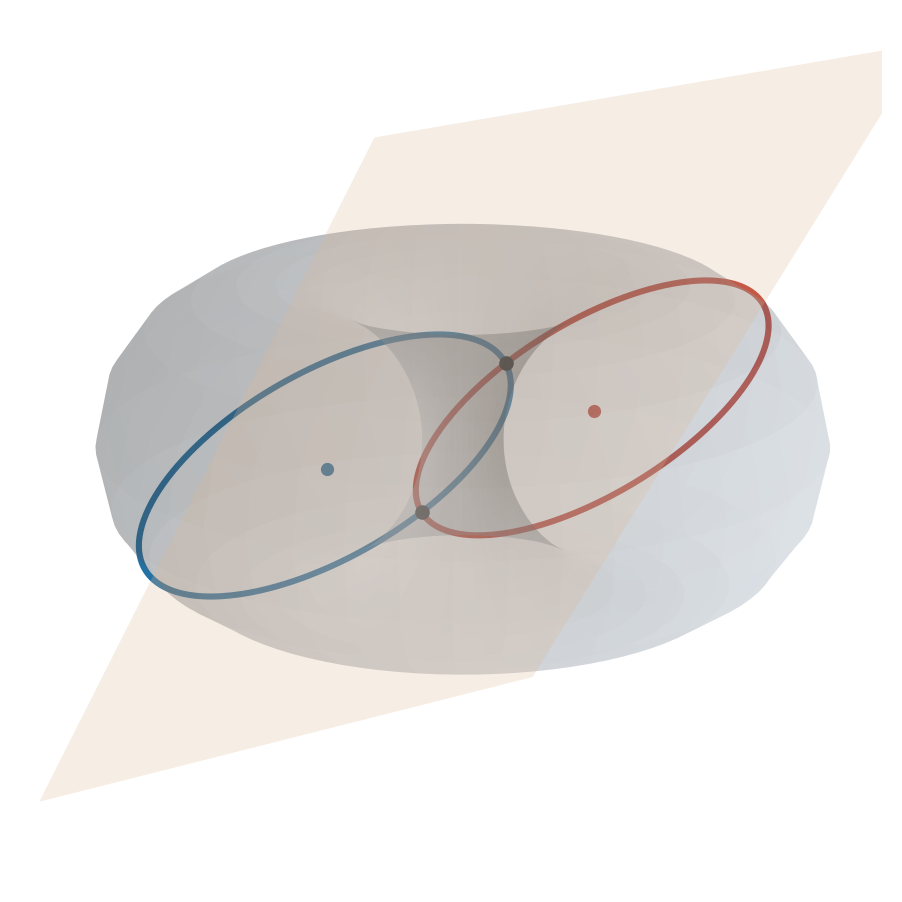
\includegraphics[width=0.92\textwidth]{fig_villarceau.png}
\caption{A ring torus with $R^2-r^2=1$, the bitangent plane $\Pi$ through its centre, the two Villarceau circles $\sigma(F_1)$ and its mirror image, of radius $R$ and centres $(0,\pm r,0)$, and the two points of tangency at distance $1$ from the centre.}
\label{fig:villarceau}
\end{figure}

\section{The meridians are Apollonian circles}\label{sec:apollonius}

As $a$ varies in $(0,1)$ the tori $T_{R,r}=\sigma(\Sigma_a)$ fill $\R^3$ minus the $x_3$-axis and the unit circle of the horizontal plane, which are the images of the fibres over the two poles. Their meridians in the half-plane $\{x_2=0,\ x_1>0\}$ are the circles
\[
M_R=\{(x_1-R)^2+x_3^2=R^2-1\},\qquad R>1 .
\]

\begin{proposition}\label{prop:apollonius}
$M_R$ is the circle of Apollonius $\{P:|P-(1,0)|=\kappa\,|P-(-1,0)|\}$ with $\kappa^2=(R-1)/(R+1)=(1-a)/(1+a)$. The circles $M_R$ form the hyperbolic pencil of circles with limit points $(\pm1,0)$, and they are orthogonal to every circle through $(1,0)$ and $(-1,0)$.
\end{proposition}

\begin{proof}
On $M_R$ we have $x_1^2+x_3^2=2Rx_1-1$, so $|P-(1,0)|^2=2(R-1)x_1$ and $|P-(-1,0)|^2=2(R+1)x_1$. The ratio is $(R-1)/(R+1)$, and $R=1/a$ gives the second expression. For the orthogonality, an inversion centred at $(-1,0)$ maps the circles $M_R$ to concentric circles about the image of $(1,0)$, and the circles through $(\pm1,0)$ to lines through that point; inversions preserve angles.
\end{proof}

The limit point $(1,0)$ is the point of the meridian half-plane on the unit circle, the image of the fibre over one pole, and the tori shrink to it as $a\to1$; as $a\to0$ they grow towards the axis. Figure~\ref{fig:meridians} shows the pencil together with the bitangent lines of one meridian.

\begin{figure}[ht]
\centering
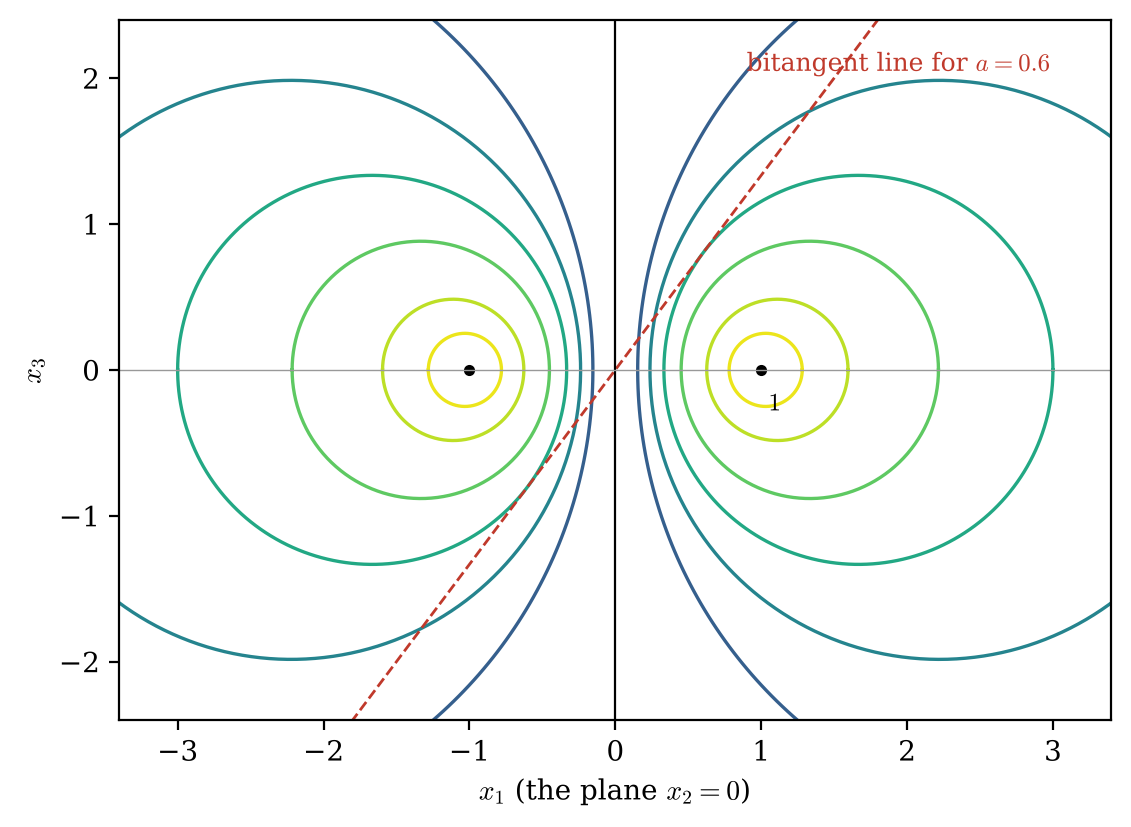
\includegraphics[width=0.8\textwidth]{fig_meridians.png}
\caption{Meridians of the tori $\sigma(\Sigma_a)$ in the half-plane $x_2=0$: the Apollonian circles with limit points $(\pm1,0)$. The line through the origin tangent to one meridian is the trace of a bitangent plane, and its point of tangency lies on the unit circle.}
\label{fig:meridians}
\end{figure}

The point of tangency of every bitangent plane lies at distance $\sqrt{R^2-r^2}=1$ from the centre, by Proposition~\ref{prop:bitangent}. So in the meridian half-plane the points of tangency of all the tori $\sigma(\Sigma_a)$ lie on the unit circle, which is the circle through the two limit points orthogonal to all the meridians; in higher dimensions Proposition~\ref{prop:twofamilies}(iii) gives the same statement with the unit $(d-2)$-sphere.
